\documentclass[11pt]{article}
\usepackage[a4paper,margin=2.2cm]{geometry}
\usepackage{amsmath,amssymb}
\usepackage{graphicx}
\usepackage{subcaption}
\usepackage{booktabs}
\usepackage{xcolor}
\usepackage{array}
\usepackage[colorlinks=true,linkcolor=blue,citecolor=blue]{hyperref}

% assets live next to this file, in reports/clipping_assets/
\graphicspath{{clipping_assets/}}

\newcommand{\code}[1]{\texttt{#1}}

\title{\textbf{Clipping \& Activation Shaping for Byzantine-Robust FL}\\[2pt]
\large Exact mechanisms and a like-for-like comparison}
\author{ByzFL\_SNN --- honest-side variance shaping study}
\date{\today}

\begin{document}
\maketitle

\begin{abstract}
This report collects, in one place, the \emph{exact} mathematical definition of every
clipping / activation-shaping mechanism implemented in the \code{activation\_clip} family,
keyed by the config name used to launch it, and then compares them on one shared benchmark
grid. Every mechanism is a \emph{honest-side} intervention (it modifies what an honest
client computes or sends, never the server aggregation), so all of them are orthogonal to
the choice of robust aggregator. We add three baselines --- the plain-ReLU CNN, a
$\tanh$ CNN, and a hard-clamped ($\mathrm{hardtanh}$) CNN --- and a spiking-network (SNN)
context comparison. Two findings stand out: (i) among fixed absolute raw-gradient caps, a
\emph{monotone dose--response} in the hardest regime (tighter cap $\Rightarrow$ more robust
at extreme heterogeneity), whose optimum shifts with the heterogeneity level; and (ii) a
clear separation between mechanisms acting on the \emph{gradient} (robust) and those acting
on the \emph{activation} (mostly ineffective, sometimes harmful even without attack).
\end{abstract}

\section{Shared experimental setup}
Unless stated otherwise, every heatmap in this report uses the identical protocol, so cells
are directly comparable across mechanisms:
\begin{itemize}\itemsep2pt
  \item \textbf{Model} \code{cnn\_mnist}: 2 conv + 2 FC, layers named
        $\{\code{\_c1},\code{\_c2},\code{\_f1},\code{\_f2}\}$, ReLU, \code{log\_softmax} head,
        \code{NLLLoss}. MNIST, SGD, lr $0.15$, momentum $0.9$, weight decay $10^{-4}$,
        batch $128$, $500$ steps, \textbf{5 seeds}.
  \item $n=10$ honest clients, $f\in\{0,1,2,3,4,5\}$ Byzantine (heatmap $x$-axis).
  \item Heterogeneity $\gamma\in\{1.0,0.66,0.33,0.0\}$ (heatmap $y$-axis; $\gamma{=}1$ near-iid,
        $\gamma{=}0$ extreme non-iid, near-disjoint classes per client).
  \item Pre-aggregation \textbf{NNM$\to$ARC}; aggregators
        \{GeometricMedian, CenteredClipping, TrMean, MultiKrum\}.
  \item Attacks: \{Optimal~ALIE~(neg1), SignFlipping, Optimal~IPM\}.
  \item Each reported cell is \code{best\_test} $=$ \emph{worst case over attacks},
        then best over aggregators --- i.e.\ the accuracy a defender is guaranteed against
        the strongest of the three attacks.
\end{itemize}
The SNN context figures (Sec.~\ref{sec:snn}) use a \emph{different} grid ($n=16$,
\code{convnet\_*}) and are therefore only internally comparable (SNN vs.\ CNN), not
cell-for-cell against the $n=10$ grid above.

\section{Two families of mechanism}
Every mechanism below is one of two kinds, distinguished by \emph{what quantity} it bounds:
\begin{description}\itemsep3pt
  \item[Activation-level] reshapes a saturating activation's forward value and/or its
    backward (surrogate) derivative. Bounds the \emph{feature} magnitude and hence,
    indirectly, the per-example gradient. Realised as a custom \code{autograd.Function}
    swapped in for ReLU (file \code{clipped\_activations.py}).
  \item[Gradient-level] bounds the L2 norm of the honest client's \emph{gradient vector}
    directly, at one of two pipeline positions (file \code{client.py}):
    \emph{raw} (on \code{.grad} right after \code{backward()}, before the momentum
    accumulator $v\!\leftarrow\!\beta v+(1-\beta)g$) or \emph{post-momentum} (on the copy
    sent to the server, leaving the internal buffer untouched).
\end{description}
The raw position is the one that can actually prevent the momentum recursion from diverging;
the post-momentum position only bounds what the aggregator sees.

\section{Exact mathematics, by config name}

\subsection{Baselines (no honest-side gradient clip)}
\paragraph{\code{cnn\_mnist} --- plain ReLU (reference).}
Standard $\mathrm{ReLU}(x)=\max(0,x)$, ordinary autograd derivative
$\mathbb{1}[x>0]$. No bound on activations or gradients. This is the reference every
mechanism is trying to improve on.

\paragraph{\code{cnn\_mnist\_tanh} --- $\tanh$ activation.}
Replaces each ReLU with $y=\tanh(x)$, a naturally saturating unit with bounded
derivative $\partial y/\partial x = 1-\tanh^2(x)\in(0,1]$. The bound is intrinsic
(no threshold to pick) and the gradient never hard-zeros.

\paragraph{\code{cnn\_mnist\_clipping\_C} --- hard-clamped ReLU ($\mathrm{hardtanh}$), $C\in\{1,2,4\}$.}
Forward is a genuine clamp $y=\mathrm{hardtanh}(x,0,C)=\min(\max(x,0),C)$ with the
\emph{true} clamp derivative:
\[
  y=\mathrm{clamp}(x,0,C),\qquad
  \frac{\partial y}{\partial x}=\mathbb{1}[0<x\le C].
\]
Above $C$ the gradient is exactly $0$ (the saturated unit stops learning). $C{=}2$ is
shown as the representative baseline.

\subsection{Activation-level, custom backward (\code{clipped\_activations.py})}
All three share the \emph{same} forward clamp $y=\mathrm{clamp}(x,0,C)$; they differ only in
the backward (surrogate) derivative.

\paragraph{\code{cnn\_mnist\_clip\_ste\_C} --- straight-through estimator, $C\in\{1,2\}$.}
\[
  y=\mathrm{clamp}(x,0,C),\qquad
  \frac{\partial y}{\partial x}=\mathbb{1}[x>0].
\]
The gradient survives \emph{everywhere} $x>0$, including above the clip (unlike hardtanh).
The forward is clamped but the backward pretends it was not.

\paragraph{\code{cnn\_mnist\_clip\_ramp\_C} --- linear ramp-down backward, $C\in\{1,2\}$, ratio $r=2$.}
Interpolates between hardtanh (hard cutoff) and STE (no cutoff): full gradient up to $C$,
then a linear decay to $0$ over $(C,rC]$:
\[
  \frac{\partial y}{\partial x}=
  \begin{cases}
    1, & 0<x\le C,\\[2pt]
    \dfrac{rC-x}{rC-C}, & C<x<rC,\\[6pt]
    0, & x\le 0 \ \text{or}\ x\ge rC.
  \end{cases}
\]
Preserves the distinction between ``slightly over'' and ``far over'' the clip.

\paragraph{\code{cnn\_mnist\_clip\_qcoord\_plain\_$0T$} --- adaptive per-pass quantile clamp, $\tau\in\{0.80,0.90\}$.}
The threshold is not hand-picked: on every forward pass it is recomputed as the
$\tau$-quantile of that layer's own activation coordinates (detached, i.e.\ treated as a
constant for backprop), so it tracks the activation distribution:
\[
  C=\mathrm{quantile}_\tau\!\big(\mathrm{flatten}(x)\big)\ \text{(detached)},\quad
  y=\mathrm{clamp}(x,0,C),\quad
  \frac{\partial y}{\partial x}=\mathbb{1}[0<x\le C].
\]
(The ``plain'' suffix is the hardtanh-style backward. An STE-backward variant was implemented
but dropped: it degraded even clean accuracy, see Sec.~\ref{sec:findings}.)

\subsection{Gradient-level, adaptive windowed quantile (\code{client.py})}
Each honest client rescales its gradient so the L2 norm does not exceed the $q$-quantile of
its own last $W$ pre-clip norms (sliding window $W{=}100$; norms are non-stationary and shrink
as training converges). With $n_t=\lVert g_t\rVert_2$ and
$\theta_t=\mathrm{quantile}_q(\{n_{t-W},\dots,n_{t-1}\})$,
\[
  g_t \;\longmapsto\;
  \begin{cases}
    g_t\cdot \theta_t/n_t, & n_t>\theta_t,\\
    g_t, & \text{otherwise.}
  \end{cases}
\]
Non-finite norms are skipped (never recorded), otherwise a single NaN would poison every
later quantile and silently disable clipping. Two positions:
\begin{itemize}\itemsep1pt
  \item \code{cnn\_mnist\_qclip\_$0Q$} ($q\in\{0.70,0.80\}$): applied \textbf{post-momentum},
        on the copy sent to the server; the momentum buffer is never rescaled (cannot stop the
        buffer itself diverging).
  \item \code{raw\_grad\_clip\_quantile} (config \code{cnn\_mnist\_rawqclip\_080}, pilot):
        same formula, applied to the \textbf{raw} gradient before the momentum accumulator ---
        the adaptive counterpart of the fixed cap below.
\end{itemize}

\subsection{Gradient-level, fixed absolute cap (raw position)}
The workhorse family. A single constant $C$ caps the raw gradient norm right after
\code{backward()} via \code{clip\_grad\_norm\_}, i.e.\ $g\mapsto g\cdot\min(1,\,C/\lVert g\rVert_2)$.
No online statistic, no SNN. The configs differ only in \emph{how $C$ is chosen}:
\begin{center}
\begin{tabular}{@{}lcl@{}}
\toprule
config & cap $C$ & how the value is obtained \\
\midrule
\code{cnn\_mnist\_gradclip\_qlow}   & $7.7$  & tightest algorithm bracket ($q_{0.90}$ of honest norms) \\
\code{cnn\_mnist\_gradclip\_calib}  & $17.6$ & calibration algorithm, $q_{0.99}$ (\code{calibrate\_clip.py}) \\
\code{cnn\_mnist\_gradclip21}       & $21$   & SNN-derived honest ceiling (reproduce baseline) \\
\code{cnn\_mnist\_gradclip\_qhigh}  & $26.7$ & loosest algorithm bracket ($q_{1.0}$ / max over $\gamma$) \\
\bottomrule
\end{tabular}
\end{center}

\paragraph{\code{cnn\_mnist\_layerclip} --- per-layer fixed caps.}
Same raw position, but a \emph{separate} cap per named module (a box constraint instead of a
single global ball), each at that layer's own offline ceiling:
\[
  C_{\code{\_c1}}=1.3,\quad C_{\code{\_c2}}=4.4,\quad C_{\code{\_f1}}=12.3,\quad C_{\code{\_f2}}=12.2,
\]
applied as \code{clip\_grad\_norm\_(module.parameters(), $C_\ell$)} for each $\ell$.

\paragraph{Self-calibrated warmup clip (\code{cnn\_mnist\_selfclip\_wW}, studied separately).}
No probe and no SNN: each client observes its own raw norm for the first $W$ steps, then
\emph{freezes} an absolute cap $C_{\text{self}}=(\max_{t\le W}n_t)\cdot m$ (margin $m$) and
clips to it forever after. Same raw position as the fixed caps; the only difference is that
$C$ is bootstrapped online from the client's own early training rather than set offline.
Reported in the companion self-clip section of \code{activation\_clip\_report.tex}.

\section{Comparison on the shared grid}
All heatmaps below are \code{best\_test} (worst-case over attacks). Read each as: how well does
this honest-side mechanism hold up as heterogeneity ($y$, top${=}$hard) and Byzantine count
($x$, right${=}$hard) increase. The easy rows ($\gamma{=}0.66,1.0$) are near-saturated for
every mechanism, so the story lives in the top two rows.

\subsection{Baselines}
\begin{figure}[h]
  \centering
  \begin{subfigure}{0.32\textwidth}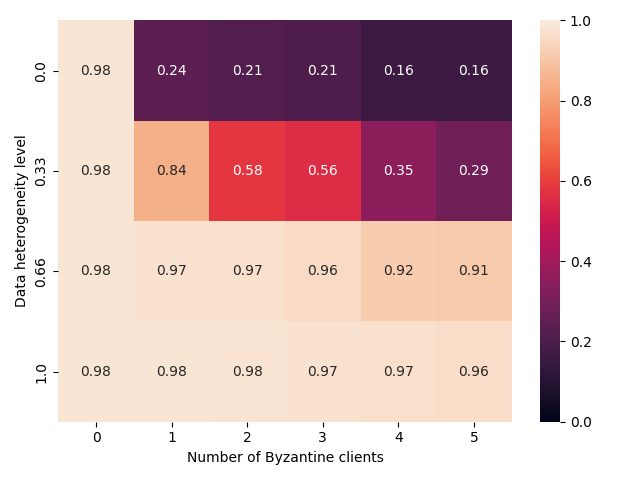
\includegraphics[width=\linewidth]{baseline_relu.png}\caption{\code{cnn\_mnist} plain ReLU}\end{subfigure}\hfill
  \begin{subfigure}{0.32\textwidth}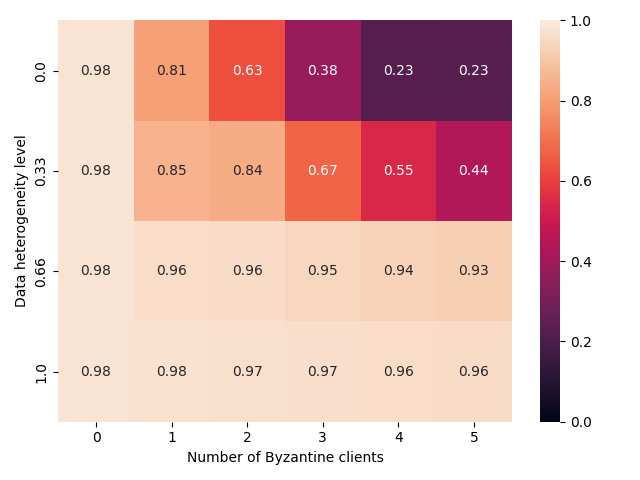
\includegraphics[width=\linewidth]{baseline_tanh.png}\caption{\code{cnn\_mnist\_tanh}}\end{subfigure}\hfill
  \begin{subfigure}{0.32\textwidth}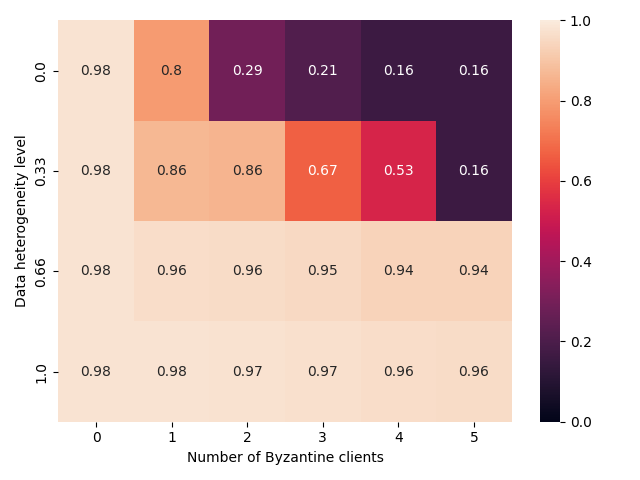
\includegraphics[width=\linewidth]{baseline_hardtanh2.png}\caption{\code{clipping\_2} hardtanh $C{=}2$}\end{subfigure}
  \caption{Baselines. Plain ReLU collapses to $0.24$ already at $\gamma{=}0,f{=}1$; the two
  bounded-activation variants ($\tanh$, hardtanh) recover the mid-heterogeneity band but
  still fall apart at the $\gamma{=}0$ wall.}
\end{figure}

\subsection{Activation-level mechanisms (custom backward)}
\begin{figure}[h]
  \centering
  \begin{subfigure}{0.32\textwidth}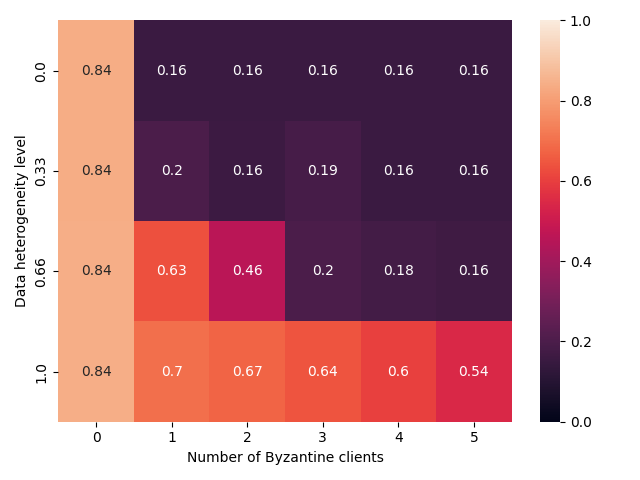
\includegraphics[width=\linewidth]{act_ste1.png}\caption{\code{clip\_ste\_1} (STE)}\end{subfigure}\hfill
  \begin{subfigure}{0.32\textwidth}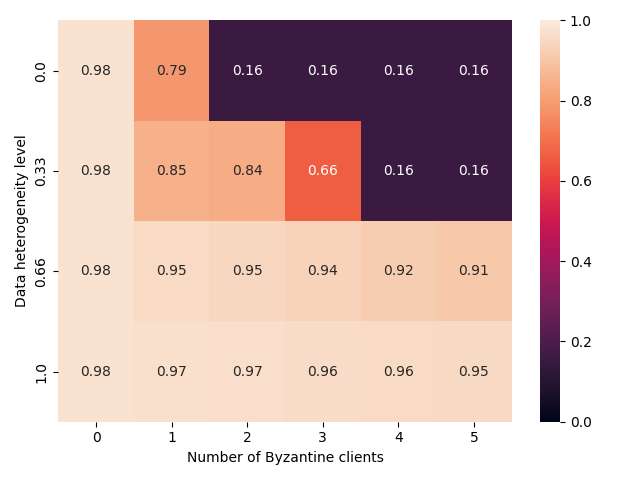
\includegraphics[width=\linewidth]{act_ramp1.png}\caption{\code{clip\_ramp\_1} ($C{=}1,r{=}2$)}\end{subfigure}\hfill
  \begin{subfigure}{0.32\textwidth}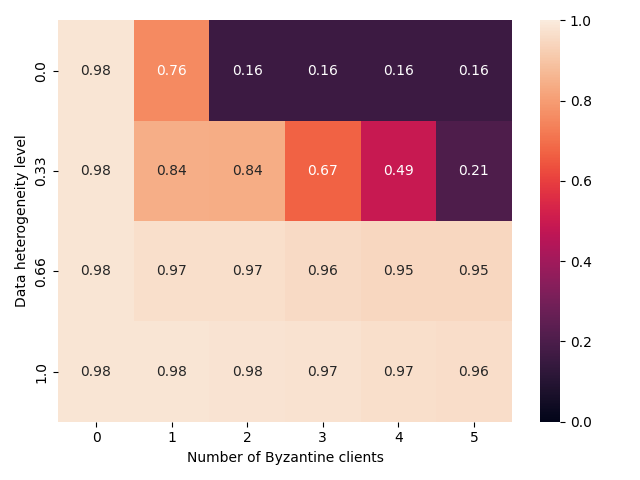
\includegraphics[width=\linewidth]{act_ramp2.png}\caption{\code{clip\_ramp\_2} ($C{=}2,r{=}2$)}\end{subfigure}
  \\[4pt]
  \begin{subfigure}{0.32\textwidth}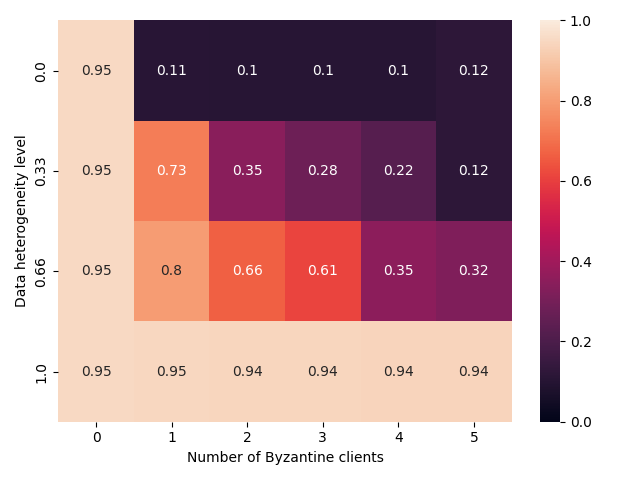
\includegraphics[width=\linewidth]{act_qcoord080.png}\caption{\code{qcoord\_plain\_080} ($\tau{=}0.80$)}\end{subfigure}\hfill
  \begin{subfigure}{0.32\textwidth}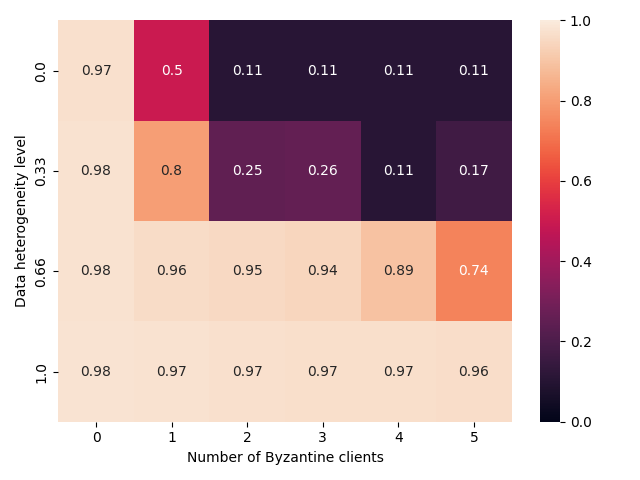
\includegraphics[width=\linewidth]{act_qcoord090.png}\caption{\code{qcoord\_plain\_090} ($\tau{=}0.90$)}\end{subfigure}\hfill
  \begin{subfigure}{0.32\textwidth}\ \end{subfigure}
  \caption{Activation-level. STE is harmful even with no attack ($0.84$ at $f{=}0$).
  Ramp recovers clean accuracy but still collapses at $\gamma{=}0,f{\ge}2$. The adaptive
  coordinate-quantile clamp is the weakest at the wall.}
\end{figure}

\subsection{Gradient-level: adaptive windowed quantile (post-momentum)}
\begin{figure}[h]
  \centering
  \begin{subfigure}{0.40\textwidth}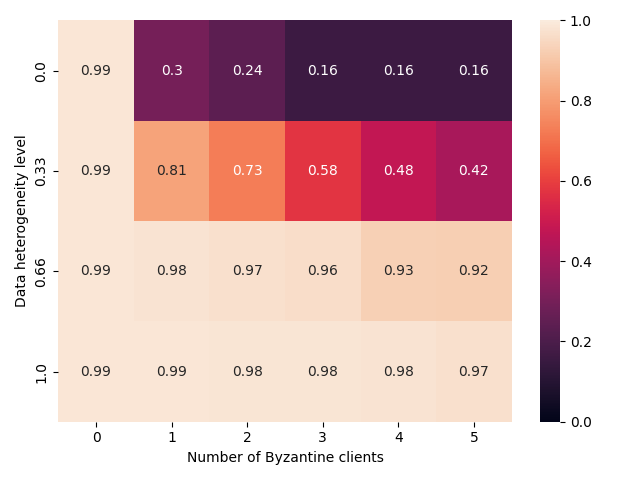
\includegraphics[width=\linewidth]{grad_qclip070.png}\caption{\code{qclip\_070} ($q{=}0.70$)}\end{subfigure}\hspace{0.04\textwidth}
  \begin{subfigure}{0.40\textwidth}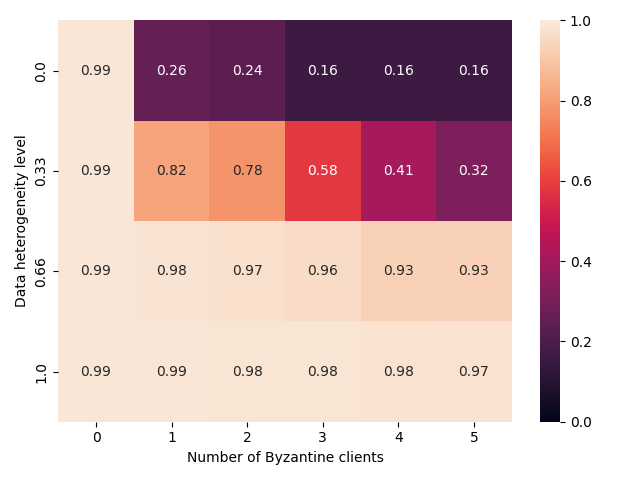
\includegraphics[width=\linewidth]{grad_qclip080.png}\caption{\code{qclip\_080} ($q{=}0.80$)}\end{subfigure}
  \caption{Adaptive quantile clip on the post-momentum vector. Strong at $\gamma{=}0.33$
  but collapses at the $\gamma{=}0$ wall (the buffer itself is never bounded).}
\end{figure}

\subsection{Gradient-level: fixed absolute raw cap (the dose--response family)}
\begin{figure}[h]
  \centering
  \begin{subfigure}{0.32\textwidth}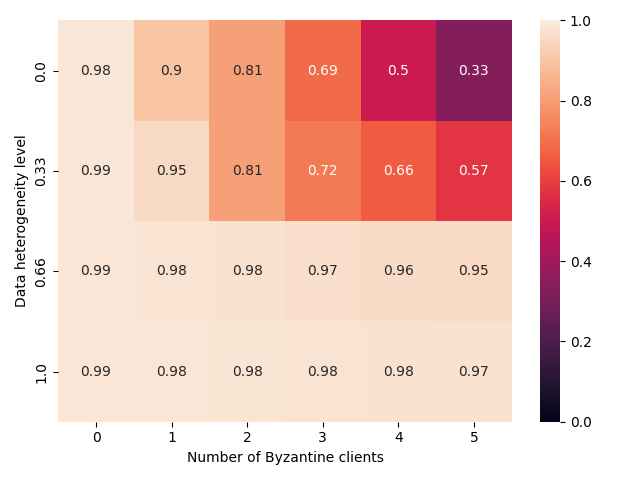
\includegraphics[width=\linewidth]{grad_qlow.png}\caption{\code{gradclip\_qlow} $C{=}7.7$}\end{subfigure}\hfill
  \begin{subfigure}{0.32\textwidth}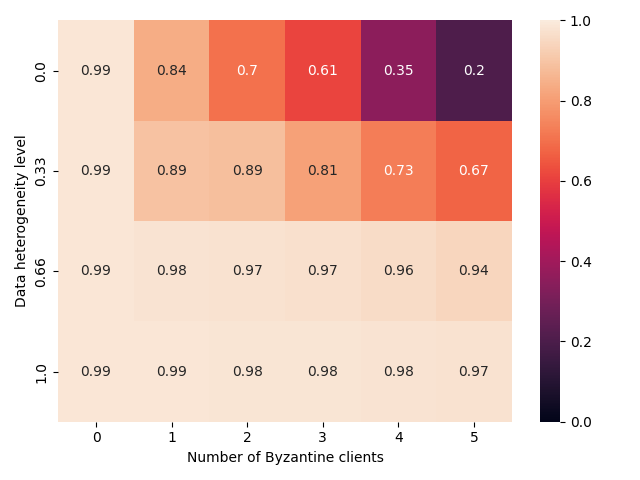
\includegraphics[width=\linewidth]{grad_calib.png}\caption{\code{gradclip\_calib} $C{=}17.6$}\end{subfigure}\hfill
  \begin{subfigure}{0.32\textwidth}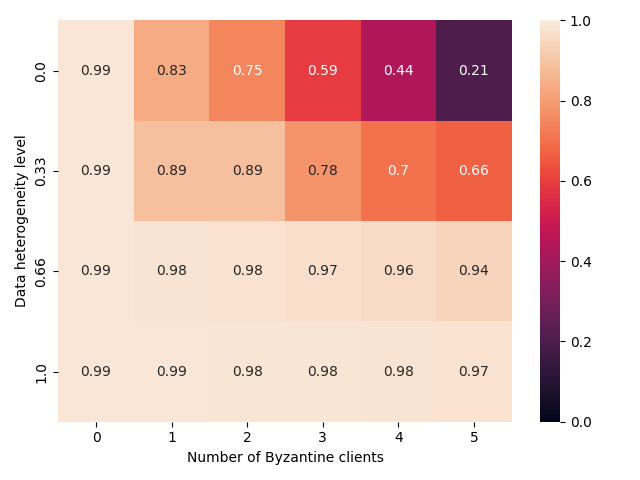
\includegraphics[width=\linewidth]{grad_clip21.png}\caption{\code{gradclip21} $C{=}21$}\end{subfigure}
  \\[4pt]
  \begin{subfigure}{0.32\textwidth}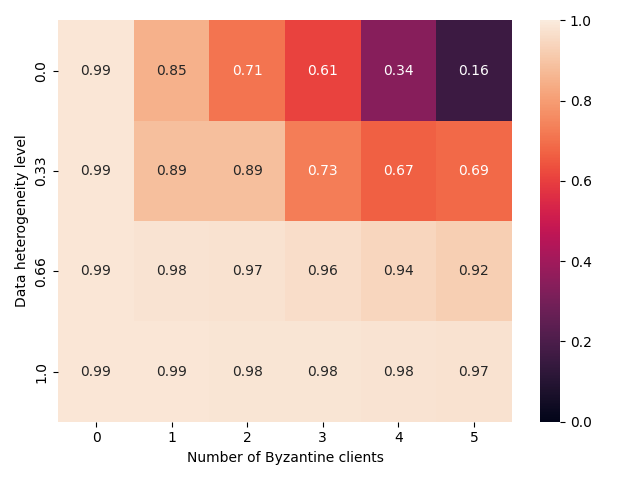
\includegraphics[width=\linewidth]{grad_qhigh.png}\caption{\code{gradclip\_qhigh} $C{=}26.7$}\end{subfigure}\hfill
  \begin{subfigure}{0.32\textwidth}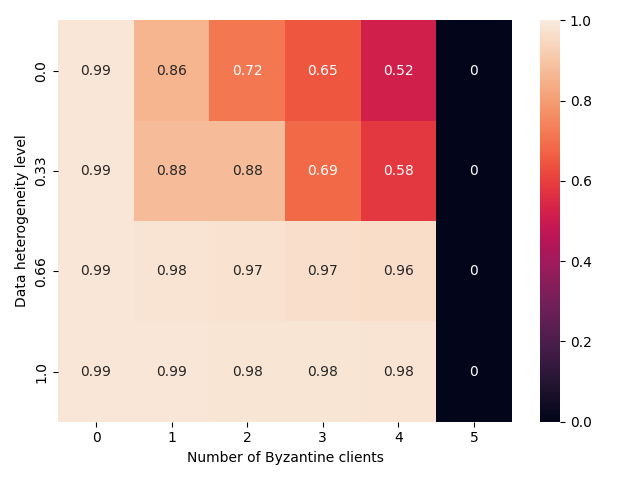
\includegraphics[width=\linewidth]{grad_layerclip.png}\caption{\code{layerclip} (per-layer)}\end{subfigure}\hfill
  \begin{subfigure}{0.32\textwidth}\ \end{subfigure}
  \caption{Fixed absolute raw-gradient caps. As $C$ tightens ($26.7\to7.7$) robustness at
  the $\gamma{=}0$ wall \emph{improves} monotonically. \code{layerclip}'s $f{=}5$ column is
  uniformly $0.00$ across every $\gamma$ (including near-iid) --- a crash, not a result
  (Sec.~\ref{sec:findings}).}
\end{figure}

\subsection{Head-to-head on the two hard rows}
Worst-case accuracy on the two heterogeneous rows (easy rows omitted --- all $\ge0.91$).
Best in each column is \textbf{bold}; the plain-ReLU reference is at the top.
\begin{center}\small
\setlength{\tabcolsep}{5pt}
\begin{tabular}{@{}ll cccccc @{}}
\toprule
& & \multicolumn{6}{c}{$f=0,1,2,3,4,5$}\\
\cmidrule(l){3-8}
mechanism & cap/param & $0$ & $1$ & $2$ & $3$ & $4$ & $5$\\
\midrule
\multicolumn{8}{@{}l}{\emph{$\gamma=0.0$ (extreme non-iid)}}\\
plain ReLU (ref) & ---        & 0.98 & 0.24 & 0.21 & 0.21 & 0.16 & 0.16\\
tanh             & ---        & 0.98 & 0.81 & 0.63 & 0.38 & 0.23 & 0.23\\
hardtanh         & $C{=}2$    & 0.98 & 0.80 & 0.29 & 0.21 & 0.16 & 0.16\\
qclip (mom.)     & $q{=}0.80$ & 0.99 & 0.26 & 0.24 & 0.16 & 0.16 & 0.16\\
\textbf{gradclip qlow} & $7.7$ & 0.98 & \textbf{0.90} & \textbf{0.81} & \textbf{0.69} & \textbf{0.50} & \textbf{0.33}\\
gradclip calib   & $17.6$     & 0.99 & 0.84 & 0.70 & 0.61 & 0.35 & 0.20\\
gradclip21       & $21$       & 0.99 & 0.83 & 0.75 & 0.59 & 0.44 & 0.21\\
gradclip qhigh   & $26.7$     & 0.99 & 0.85 & 0.71 & 0.61 & 0.34 & 0.16\\
layerclip        & per-layer  & 0.99 & 0.86 & 0.72 & 0.65 & \textbf{0.52} & 0.00\\
\midrule
\multicolumn{8}{@{}l}{\emph{$\gamma=0.33$ (moderate non-iid)}}\\
plain ReLU (ref) & ---        & 0.98 & 0.84 & 0.58 & 0.56 & 0.35 & 0.29\\
tanh             & ---        & 0.98 & 0.85 & 0.84 & 0.67 & 0.55 & 0.44\\
hardtanh         & $C{=}2$    & 0.98 & 0.86 & 0.86 & 0.67 & 0.53 & 0.16\\
qclip (mom.)     & $q{=}0.80$ & 0.99 & 0.82 & 0.78 & 0.58 & 0.41 & 0.32\\
gradclip qlow    & $7.7$      & 0.99 & \textbf{0.95} & 0.81 & 0.72 & 0.66 & 0.57\\
\textbf{gradclip calib} & $17.6$ & 0.99 & 0.89 & \textbf{0.89} & \textbf{0.81} & \textbf{0.73} & 0.67\\
gradclip21       & $21$       & 0.99 & 0.89 & \textbf{0.89} & 0.78 & 0.70 & 0.66\\
gradclip qhigh   & $26.7$     & 0.99 & 0.89 & \textbf{0.89} & 0.73 & 0.67 & \textbf{0.69}\\
layerclip        & per-layer  & 0.99 & 0.88 & 0.88 & 0.69 & 0.58 & 0.00\\
\bottomrule
\end{tabular}
\end{center}

\section{Findings}\label{sec:findings}
\begin{enumerate}\itemsep4pt
  \item \textbf{Gradient-level $\gg$ activation-level.} Bounding the gradient norm directly
    is far more effective than any activation reshaping. At $\gamma{=}0,f{=}1$ the plain CNN
    is $0.24$; a fixed raw cap lifts it to $0.83$--$0.90$, whereas STE ($0.16$), the adaptive
    coordinate-quantile clamp ($0.11$) and the post-momentum \code{qclip} ($0.26$) barely move
    it. The activation is simply too indirect a handle on gradient variance.
  \item \textbf{Monotone dose--response in the hard regime.} Among the fixed absolute caps,
    the \emph{tighter} the cap the better at the $\gamma{=}0$ wall: at $f{=}5$,
    $C{=}7.7$ gives $0.33$ vs $0.16$ for $C{=}26.7$ (double); the ordering
    $7.7>21\approx17.6>26.7$ holds across $f{=}3,4,5$. The dominant robustness lever is
    ``clip hard in absolute terms,'' \emph{not} ``calibrate to the honest ceiling'' --- the
    same signal seen in the self-clip $W{=}1$ vs $W{=}50$ comparison.
  \item \textbf{But the optimum shifts with $\gamma$ --- no free lunch.} At $\gamma{=}0.33$
    the tightest cap costs accuracy in the mid-$f$ band ($C{=}7.7$ gives $0.81$ at $f{=}2$
    vs $0.89$ for the looser caps), and \code{calib}~($17.6$) is the best there. So the
    cap$\leftrightarrow$robustness curve has a heterogeneity-dependent optimum: aggressive at
    the extreme-non-iid wall, moderate at intermediate heterogeneity. This is exactly the
    ``honest-side intervention as a tunable robustness knob'' thesis, with a concrete trade-off.
  \item \textbf{STE is actively harmful.} \code{clip\_ste\_1} tops out at $0.84$ even with
    \emph{no} attack ($f{=}0$), confirming why the STE-backward quantile variant was dropped:
    letting the gradient survive above the clip destabilises clean training on MNIST.
  \item \textbf{\code{layerclip} $f{=}5$ is a crash, not a result.} Its entire $f{=}5$ column
    is $0.00$ for every $\gamma$, including near-iid $\gamma{=}1.0$ where $f{=}4$ is still
    $0.98$. This is a divergence/NaN or a missing-run artefact at $f{=}5$, not a gradual
    robustness failure --- most likely the very tight \code{\_c1}$=1.3$ conv cap interacting
    with the $f{=}5$ setting. It must be re-run/verified before \code{layerclip} is compared
    at $f{=}5$; the $f\le4$ cells are consistent with the rest of the family.
\end{enumerate}

\section{SNN context (different grid)}\label{sec:snn}
For completeness, the spiking-vs-conventional comparison from the direct-input study.
\textbf{Caveat:} this grid uses $n=16$ honest clients and the \code{convnet\_*} architecture
(not the $n=10$ \code{cnn\_mnist} above), and a slightly different ALIE variant, so these two
panels are comparable to \emph{each other} but not cell-for-cell to the main grid. They are
included because the surrogate-gradient design of an SNN is the same idea --- shaping a
saturating unit's derivative so honest-gradient statistics stay bounded --- transplanted from
the spike to the ReLU.
\begin{figure}[h]
  \centering
  \begin{subfigure}{0.44\textwidth}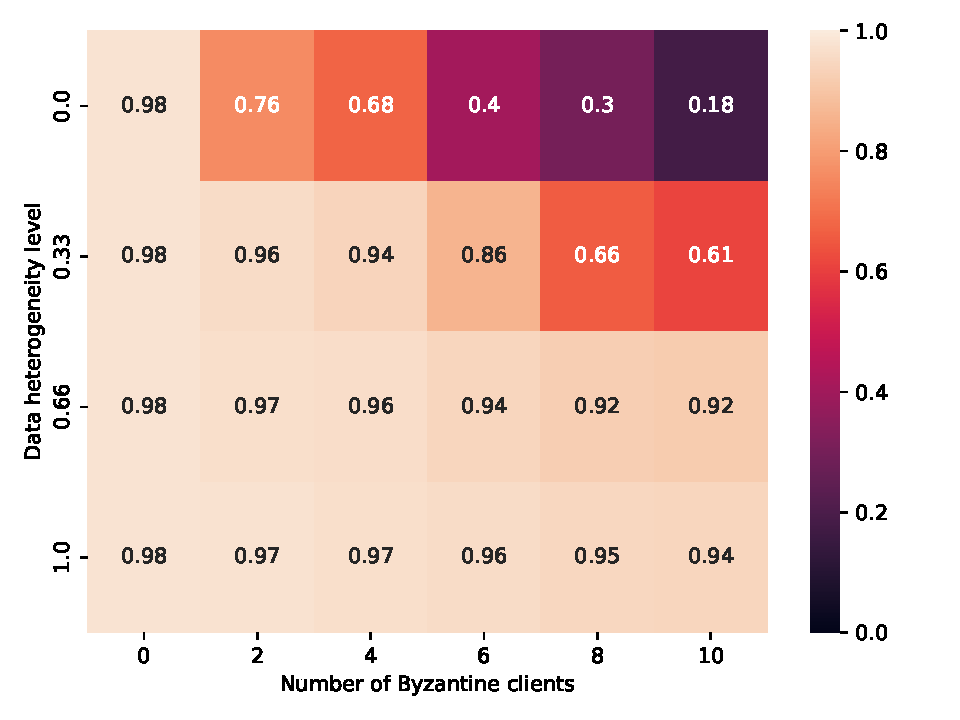
\includegraphics[width=\linewidth]{ctx_cnn_n16.pdf}\caption{\code{convnet\_cnn} ($n{=}16$)}\end{subfigure}\hspace{0.04\textwidth}
  \begin{subfigure}{0.44\textwidth}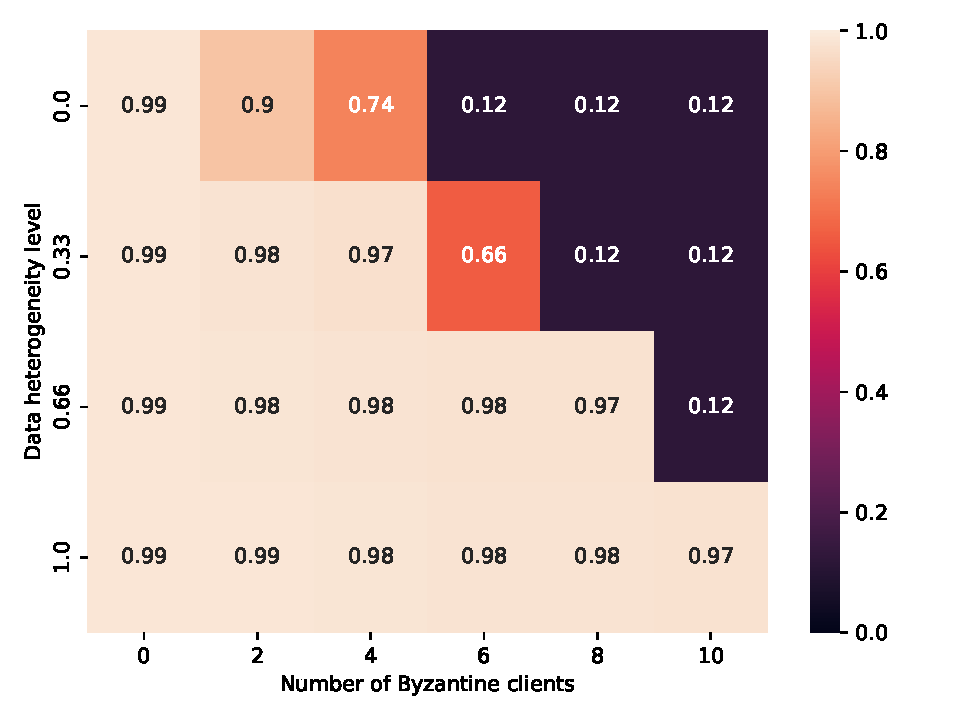
\includegraphics[width=\linewidth]{ctx_snn_n16.pdf}\caption{\code{convnet\_snn} ($n{=}16$)}\end{subfigure}
  \caption{Conventional CNN vs.\ SNN on the direct-input $n{=}16$ grid (\code{best\_test},
  worst-case over attacks). Same protocol otherwise; intended as qualitative context for the
  ``surrogate-gradient = honest-side variance shaping'' framing.}
\end{figure}

\section*{Reproducing the figures}
Every panel is \code{best\_test\_\dots.png} copied into \code{reports/clipping\_assets/}.
Raw results live under \code{results/activation\_clip/<config>/} (RCP PVC
\code{/mnt/dcl/scratch/activation\_clip/}); regenerate heatmaps with
\code{plot\_activation\_clip\_results.py --configs <config>}. Note the two-pod gamma-split
caveat: after a split A/B run, patch each \code{results\_directory/config.json}'s
\code{distribution\_parameter} back to the full $\gamma$ list before plotting (the heatmap
reader takes its rows from that field, not from the files on disk) --- see
\code{run\_gradclip\_plots.sh}.

\end{document}
